%!TEX root = paper.tex
%%%%%%%%%%%%%%%%%%%%%%%%%%%%%%%%%%%%%%%%%%%%%%%%%%%%%%%%%%%%%%%%%%%%%%%%%%%%%%%%
\section{Game Services and Data}
\label{sec:background}

This section aims to cover all basic information on Cloud Gaming and their business models. It also briefly introduces the employed datasets.

%%%%%%%%%%%%%%%%%%%%%%%%%%%%%%%%%%%%%%%%%%%%%%%%%%%%%%%%%%%%%%%%%%%%%%%%%%%%%%%%
\subsection{Service Costs of Gaming Platforms}

To evaluate the costs and benefits of individual gaming platforms, one should first take a look at the vastly different price models --- as well as the supporting competitive ecosystem surrounding them --- these services offer to their customers. For this investigation only currently active services, Cloud and otherwise, are examined which narrows the number of services considerable. The information presented here was collected in February 2016 and is subject to change. All costs shown here are from an European, specifically German, perspective. If a product is not available in this region, the prices are converted accordingly to the current exchange rates.


\subsubsection{Video Game Consoles}

One of the classical approaches to video games is using dedicated consoles with physical copies of a game bought at a retailer. The price for (non-portable) consoles varies but usually lies between \SI{300}[\EUR] and \SI{400}[\EUR] for the latest console generation, i.e. currently \textit{Wii U}, \textit{PlayStation 4}, and \textit{Xbox One}. New, major game releases are mostly priced at either \SI{60}[\EUR] or \SI{70}[\EUR]. The decline in price is rather slow for individual console games, often only happening over the course of several years.

In recent years retail stores have been more and more complemented with each console's proprietary digital distribution service, also the latest game at the full price. These official stores are usually the only vendor for digital game codes, meaning that there will be no competition that quickly reduces prices.

In order to utilize a game's multiplayer component, some services require you to opt in to a subscription, dubbed, e.g. \textit{PlayStation Plus} or \textit{Xbox Live Gold}, with annual prices of \SI{50}[\EUR] and \SI{60}[\EUR] respectively. These services do however generally offer a monthly rotating palette of (older or smaller) game titles included in the subscription.

% \paragraph{Historical Example: OnLive}


\subsubsection{The PC Gaming Ecosystem}

The rise of easy-to-use digital distribution platforms and the independent (i.e. ``indie'') game scene a few years back reinvigorated PC gaming. Today, PC gaming is dominated by large digital marketplaces, and \steam in particular. The platform, with about $10$ million concurrent users at every time of day, has fully embraced its digital and online-only nature and periodically offers large (seasonal) sales of recent games at greatly reduced prices (rebates of 75\% for a year-old game are not uncommon). 

In addition, many resellers offer digital codes for other platforms, often at much lower prices. Alternative storefronts, entirely independent of \steam, also exist, such as \textit{GOG}\footnote{\url{https://www.gog.com/}}, and enrich the competition even more.

Another recent trend are game bundles, especially prevalent in indie games, which bundle together a number of games for either a low price or, more commonly, with a pay-what-you-want model with parts of the money going to charities. \textit{Humble Bundle}\footnote{\url{https://www.humblebundle.com/}} is a prominent example for this. The official prices for new major releases on PC are comparable to that of console titles. However, due to the competition the street prices are significantly lower even at launch, and also drop more quickly.

The barrier to entry to PC gaming is a bit steeper than for consoles, albeit with increased flexibility and longevity. Hardware viable for PC gaming starts at about \SI{500}[\EUR] but has practically no upper limit for enthusiasts. The main spender will usually be the \gls{GPU}, often surpassing the \acrshort{CPU} in its performance impact in today's games by far.

%recurring bundles/subscriptions (humble monthly)
%	console/netflix similarities

% Steam Sales:
% Large seasonal sales (christmas, summer, lunar new year, halloween, fall, spring, ...) of many/most games on the platform usually rebates of 50\% and up.
% Weekly sales
% Daily sales
% Weekend sales
% Free weekends


\subsubsection{Geforce Now}

\textit{Geforce NOW}\footnote{\url{http://shield.nvidia.com/game-streaming-with-geforce-now}} is a Cloud Gaming service by NVIDIA available in North America as well as some European countries. In Germany the service currently offers access to $68$ PC titles for a monthly subscription fee of \SI{10}[\EUR]. The more prominent and recent $19$ of those titles however require an additional one-time payment between \SI{13}[\EUR] and \SI{60}[\EUR]. The service is delivered from six specialized data center locations, with Dublin and Frankfurt responsible for Europe.

The requirements to use this service are rather steep, demanding \SI{50}{\mega\bit\per\second} for a full 1080p60\footnote{\label{foot:rate}Please note: This frame rate of \SI{60}{\hertz} represents the rate of the video encoder and not the game's actual frame rate, which might be considerably lower depending on the complexity of the game.} stream (\SI{10}{\mega\bit\per\second} in order to use the service at all) and a maximum \acrshort{RTT} of \SI{60}{\milli\second} to one of the data centers. In addition, streaming is exclusive to one of NVIDIA's \textit{SHIELD} devices which start at \SI{200}[\EUR].

% Started in parts of Europe in Q4/2015


\subsubsection{Playstation Now}

In the absence of backwards compatibility in the latest PlayStation generation, the \textit{PlayStation Now} service was put in place to stream titles from the PlayStation 2 and 3 generation to the current iteration of Sony's consoles. It is currently available in North America and the UK, with a closed beta running in some other European countries as well as Japan.

Both the offered titles as well as the precise pricing vary from country to country. As stated this work will focus on the European perspective. For the UK, about $150$ titles are available. A large portion of them is included in the subscription service, incurring a monthly fee of about \SI{17}[\EUR]. All titles are also available through a separate rental service, costing about \SI{4}[\EUR] for \SI{48}{\hour} of access, and \SI{10}[\EUR] for a week. This is in addition for the device cost, as the service is only available to the PlayStation 4 and 3 consoles as well as some select Sony TVs and other devices (which would however necessitate the purchase of a game controller).

The streaming itself is performed at a resolution of 720p60\cref{foot:rate} requiring a \SI{5}{\mega\bit\per\second} connection. Reports on the video quality have been rather mixed.\footnote{\url{http://www.eurogamer.net/articles/digitalfoundry-2015-hands-on-with-playstation-now}} Sony is also reportedly using specialized hardware, adopted from regular PlayStation 3s, on their server side, effectively eliminating any chance for multi-purpose uses of these devices.

% cost and some more infos:
% http://www.pocket-lint.com/news/126394-playstation-now-subscription-service-comes-to-the-uk-what-is-it-and-how-can-you-get-it

% (US/UK only?) Deuschlandbeta seit ~Q4/2015



%%%%%%%%%%%%%%%%%%%%%%%%%%%%%%%%%%%%%%%%%%%%%%%%%%%%%%%%%%%%%%%%%%%%%%%%%%%%%%%%
\subsection{Gaming Measures and Datasets}

The leading question for the user side of the cost-benefit analysis is: ``How can we properly estimate the value a user gets from a specific service?'' with an additional question of ``What is the definition of value in this context?''. To answer these some means to meter user engagement is required, as this represents the core of those questions. Simply counting the number of games available for a specific service or for a specific amount of money may be the easiest value metric but may also fall short, as the enjoyment of a specific game can be very subjective.

However, there are still a number of metrics independent of ones own subjective opinion that can give a more objective impression of the popularity and the value of individual titles. Both these attributes usually play a role in one's decision to play a certain game. In order to investigate such metrics, data had to be collected from various sources and merged into a consistent data base. All the code, data as well as this paper itself can be found in public code repositories\footnote{The main repository can be found at \url{https://github.com/mas-ude/cost-of-cloud-gaming}} in the interest of repeatability and reproducibility. The following paragraphs describe the individual sets.

%!TEX root = paper.tex

\begin{table}
\caption{Metadata for the \steam, \metacritic, \hltb, \psnow, and \gfnow datasets. Records with a * note include games from other platforms than PC, PlayStation, and GeForce Shield.}
\label{tab:dataset-metadata}
\centering
\begin{tabu}{X[1.5]|X[r]|X[0.7,r]|X}
\toprule
Product & Date generated & \# of records & Method of generation\\
\midrule
\steam & 2015-07-14 & \num{5996} & Steam \& SteamSpy\\
\steam & 2015-10-30 & \num{6769} & Steam \& SteamSpy\\
\steam & 2016-02-06 & \num{7749} & Steam \& SteamSpy\\
\psnow & 2016-02-09 & \num{190} & Official list\\
\gfnow & 2016-02-12 & \num{69} & Manual screen scraping\\
\metacritic & 2016-03-02 & * \num{46197} & Web scraping\\
\hltb & 2016-03-01 & * \num{18433} & Web scraping\\
\bottomrule
\end{tabu}
\end{table}

%!TEX root = paper.tex

\begin{table*}
\centering
\caption{Overview of datasets. Values with * are 99th percentiles chosen due to unrealistically large outliers.}
\label{tab:dataset-stats}
\begin{tabular}{c|c|r|r|r|r|r|r}
Dataset & Metric & Mean & Min & 1Q & Median & 3Q & Max\\
\hline
\hline
\steam & Number of records & \num{7749} & -- & -- & -- & -- & -- \\
\steam & Owners & \num{218112} & \num{0} & \num{4831} & \num{21740} & \num{107299} & \num{58666968} \\
\steam & players 2weeks & \num{9064} & \num{0} & \num{0} & \num{509} & \num{1526} & \num{7860554} \\
\steam & players forever & \num{138322} & \num{0} & \num{1780} & \num{9408} & \num{51997} & \num{58666968} \\
\steam & Average playtime (forever) & \num{507} & \num{0} & \num{93} & \num{200} & \num{429} & \num{45540} \\
\steam & Median playtime (forever) & \num{246} & \num{0} & \num{36} & \num{101} & \num{216} & \num{67538} \\
\steam & average 2weeks & \num{144} & \num{0} & \num{0} & \num{48} & \num{173} & \num{11387} \\
\steam & median 2weeks & \num{126} & \num{0} & \num{0} & \num{35} & \num{128} & \num{11387} \\
\steam & Price & \num{564} & \num{-1.26} & \num{0.99} & \num{3.39} & \num{7.49} & \num{119.00} \\
\hline
\psnow & Number of records & \num{252} & -- & -- & -- & -- & -- \\
\psnow & Rental fee for 4 hours & \num{3.02} & \num{1.99} & \num{1.99} & \num{2.99} & \num{2.99} & \num{22.99} \\
\psnow & Rental fee for 7 days & \num{5.48} & \num{1.99} & \num{3.99} & \num{4.99} & \num{5.99} & \num{14.99} \\
\psnow & Rental fee for 30 days & \num{8.40} & \num{3.99} & \num{5.99} & \num{6.99} & \num{7.99} & \num{22.99} \\
\psnow & Rental fee for 90 days & \num{12.57} & \num{3.99} & \num{7.99} & \num{8.99} & \num{14.99} & \num{49.99} \\
\hline
\gfnow & Number of records & \num{68} & -- & -- & -- & -- & -- \\
\gfnow & Price & \num{6.98} & \num{0} & \num{0} & \num{0} & \num{13.99} & \num{59.99} \\
\hline
\metacritic & Number of records & \num{45803} & -- & -- & -- & -- & -- \\
\metacritic & User score & \num{6.9} & \num{0} & \num{6.2} & \num{7.3} & \num{8.1} & \num{9.3} \\
\metacritic & Score & \num{69} & \num{8} & \num{62} & \num{72} & \num{79} & \num{96} \\
\hline
\hltb & Number of records & \num{18129} & -- & -- & -- & -- & -- \\
\hltb & Main story length & \num{26} & \num{0.02} & \num{2.5} & \num{6} & \num{12} & * \num{94} \\
\hltb & Main extra length & \num{21} & \num{0.08} & \num{5} & \num{10} & \num{20} & * \num{126} \\
\hltb & Completionist length & \num{28} & \num{0.03} & \num{5} & \num{13} & \num{29} & * \num{250} \\
\hltb & Combined length & \num{13} & \num{0.02} & \num{3} & \num{8} & \num{15} & \num{420} \\
\end{tabular}
\end{table*}

\todo[inline]{PZ: Viele daten, aber welche plattform ist die beste?}


%%%%%%%%%%%%
\subsubsection{Game Prices and Ownership}

An initial grasp of the popularity of individual titles can often be derived from its price as well as the number of owners. Few platforms however publish sales numbers, though a few recurring studies on retail sales exist. For this work however, data from the \steam platform was used\footnote{\url{https://github.com/mas-ude/steam-data-stats}}. Using the official \acrshort{REST} \acrshort{API} the name and the current price of each game was fetched at three different points of time. The influence of sales periods can be easily observed in the \acrshort{CDF} of prices in Fig. \ref{fig:steam-prices}, where the data from February was collected during \steam's Lunar New Year Sale.

\begin{figure}[!t]
	\centering
	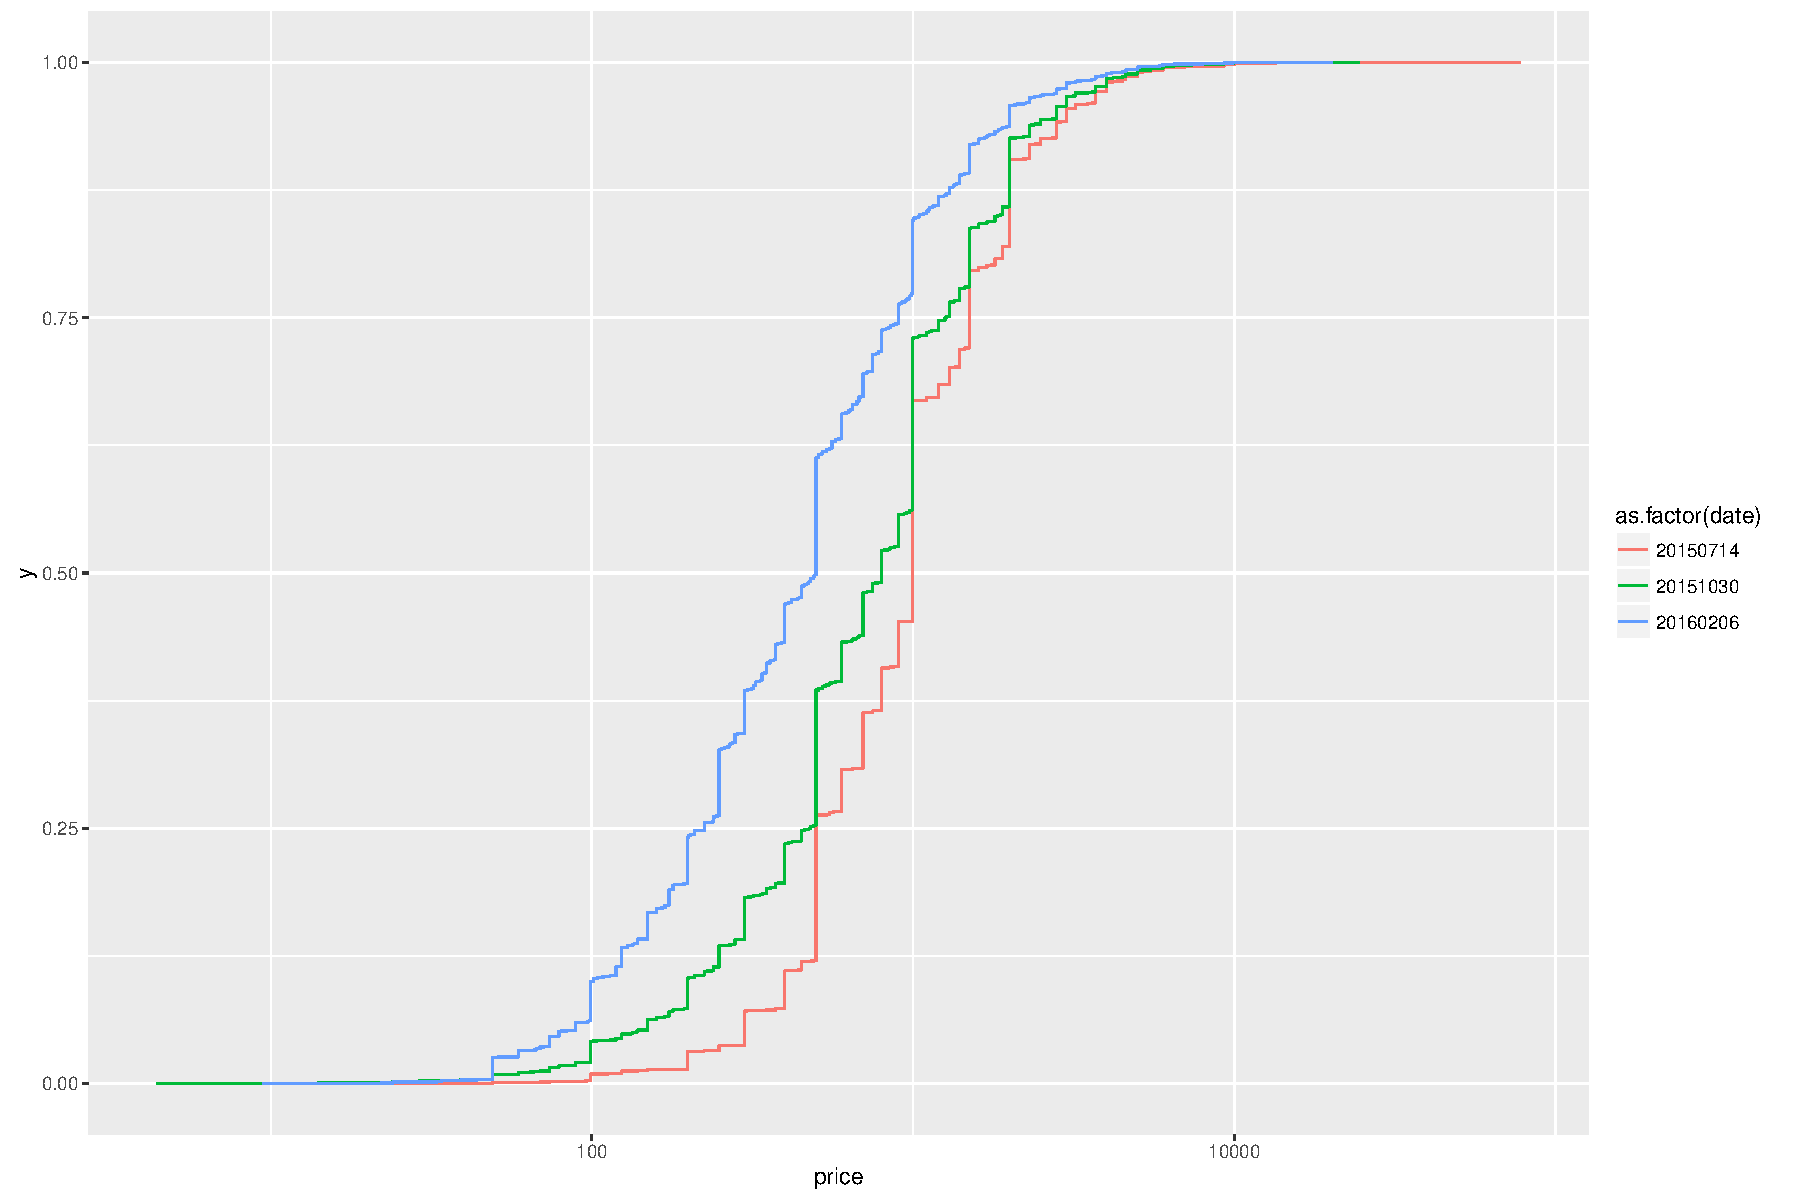
\includegraphics[width=1.0\columnwidth]{images/steam-prices.pdf}
	\caption{CDF of games on the \steam platform at three distinct dates. The February data was collected in a sales period.}
\label{fig:steam-prices}
\end{figure}

This was combined with \acrshort{API}-data from the 3rd-party Web site SteamSpy\footnote{\url{https://steamspy.com}}. This site parses the portion of publicly visible \steam user profiles and from this estimates statistics on the size of the playerbase and the time each player spends with a title. Furthermore, the site provides a heuristic projection of the total number of owners of each listed title on \steam. Using this data also immediately makes evident a relationship between the price category of a game and the average time it's being played (cf. Fig.~\ref{fig:steam-cost-vs-playtime-violin}). Free (but especially free-to-play titles with monetization options other than an upfront payment) titles seem to occupy a special position as no prevalence for specific playtimes is visible.

\todo[inline]{Ist ``free'' auch in-app Purchase Zeug?}

\begin{figure}[!t]
	\centering
	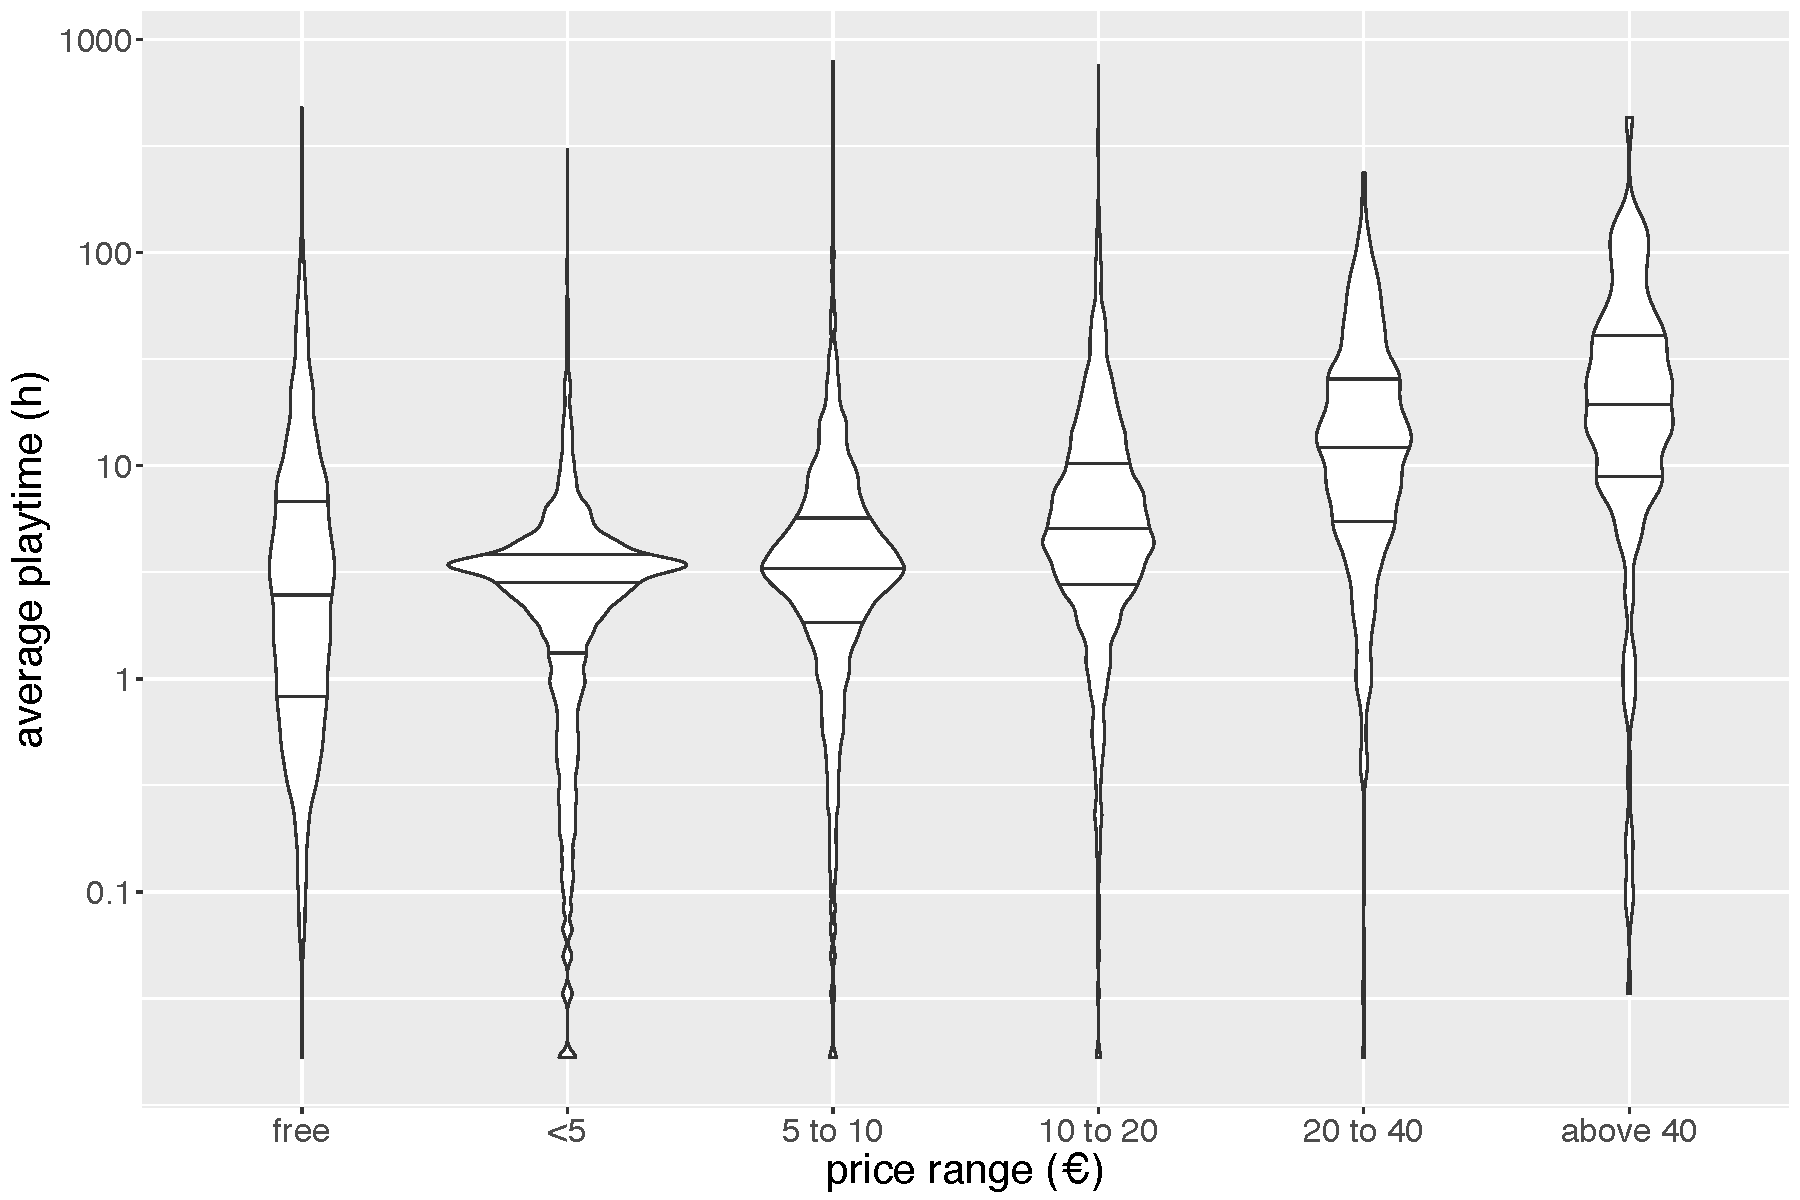
\includegraphics[width=1.0\columnwidth]{images/steam-cost-vs-playtime-non-sale.pdf}
	\caption{Violin plot of the average playtime of \steam games, broadly categorized by their prices.}
\label{fig:steam-cost-vs-playtime-violin}
\end{figure}



Due to the strong popularity of \steam in PC gaming (even physical retail copies often require using the service nowadays) this set also gives a good general overview of the dimensions of PC gaming in general.


%%%%%%%%%%%%
\subsubsection{Game Lengths}

While the previous dataset included numbers on the average playtime, but this is not necessarily representative of the length of one ``playthrough'' of a game. The latter might be another indicator of the amount (albeit not the quality) of content a game offers. To encompass this, data from the site \hltb\footnote{\url{http://howlongtobeat.com/}} was collected\footnote{\url{https://github.com/mas-ude/gamelengths-scraper}}. This site allows for manual reporting of playthrough times of games on any platform. Times are separated into different play styles (e.g. ``main story'' or ``completionist'') and only an aggregated time is shown. For this analysis only the average playtime of all play styles is taken into account. It should however be stressed again, that this is a self-reporting site without strong validity checks, which has to be considered when contemplating the accuracy of the data.

\begin{figure}[!t]
	\centering
	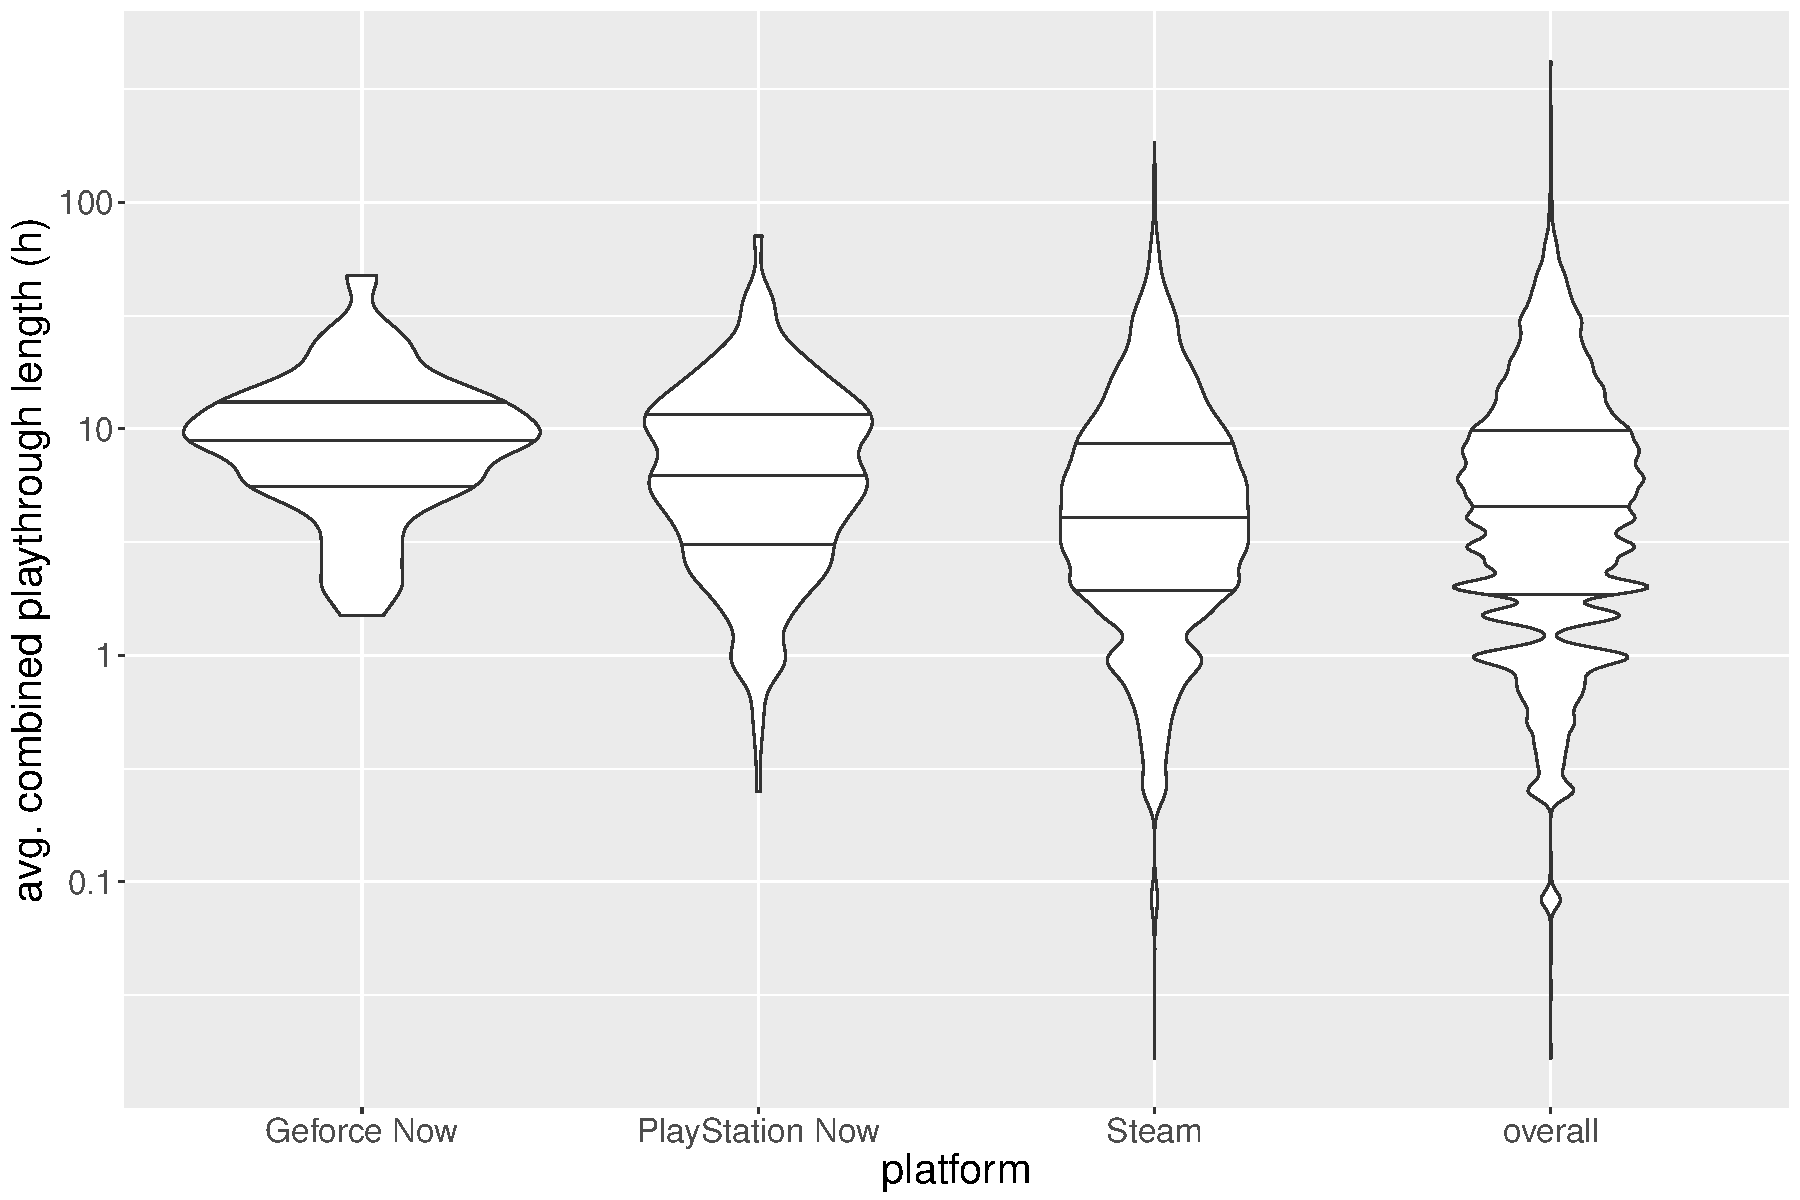
\includegraphics[width=1.0\columnwidth]{images/gamelengths-by-platform-violin.pdf}
	\caption{Violin plot of the average game lengths over all play styles and separated for the investigated platforms as recorded on \hltb.}
\label{fig:gamelengths-violin}
\end{figure}

Nonetheless, the distribution of game lengths from this set can still be worth to look at in the context of putting value to games for consumers of different platforms. As seen in Figure~\ref{fig:gamelengths-violin} the play lengths vary greatly, with the median at \SI{7.5}{\hour} and a long tail of play times reaching \SI{420}{\hour}.

%Game lengths can not only serve as an indicator of the amount of content a game has to offer, but can also serve as an engagement metric to estimate a user's amount of satisfaction. More fitting engagement metrics could also be employed.


%%%%%%%%%%%%
\subsubsection{Review Scores}

A final indirect measure of value and user satisfaction are review score as given by professional gaming media outlets. The largest dataset of such scores is available through Metacritic\footnote{\url{http://www.metacritic.com/}} and also included for this examination\footnote{\url{https://github.com/mas-ude/metacritic_scraper}}.

This set covers all gaming platforms, current and historic. The review scores are aggregated to a single average scores of $0$--$100$, although some internal weighing factors are applied, signifying the importance of some media outlets over others.

The exact release date of every title is also included, leading to another possible engagement metric: the game's age. Barring some highly favored classic titles, more recent games are usually much more popular than older ones.


% TODO: include or compare with data from opencritic.com as soon as their API is public/usable

% \begin{figure}[!t]
% 	\centering
% 	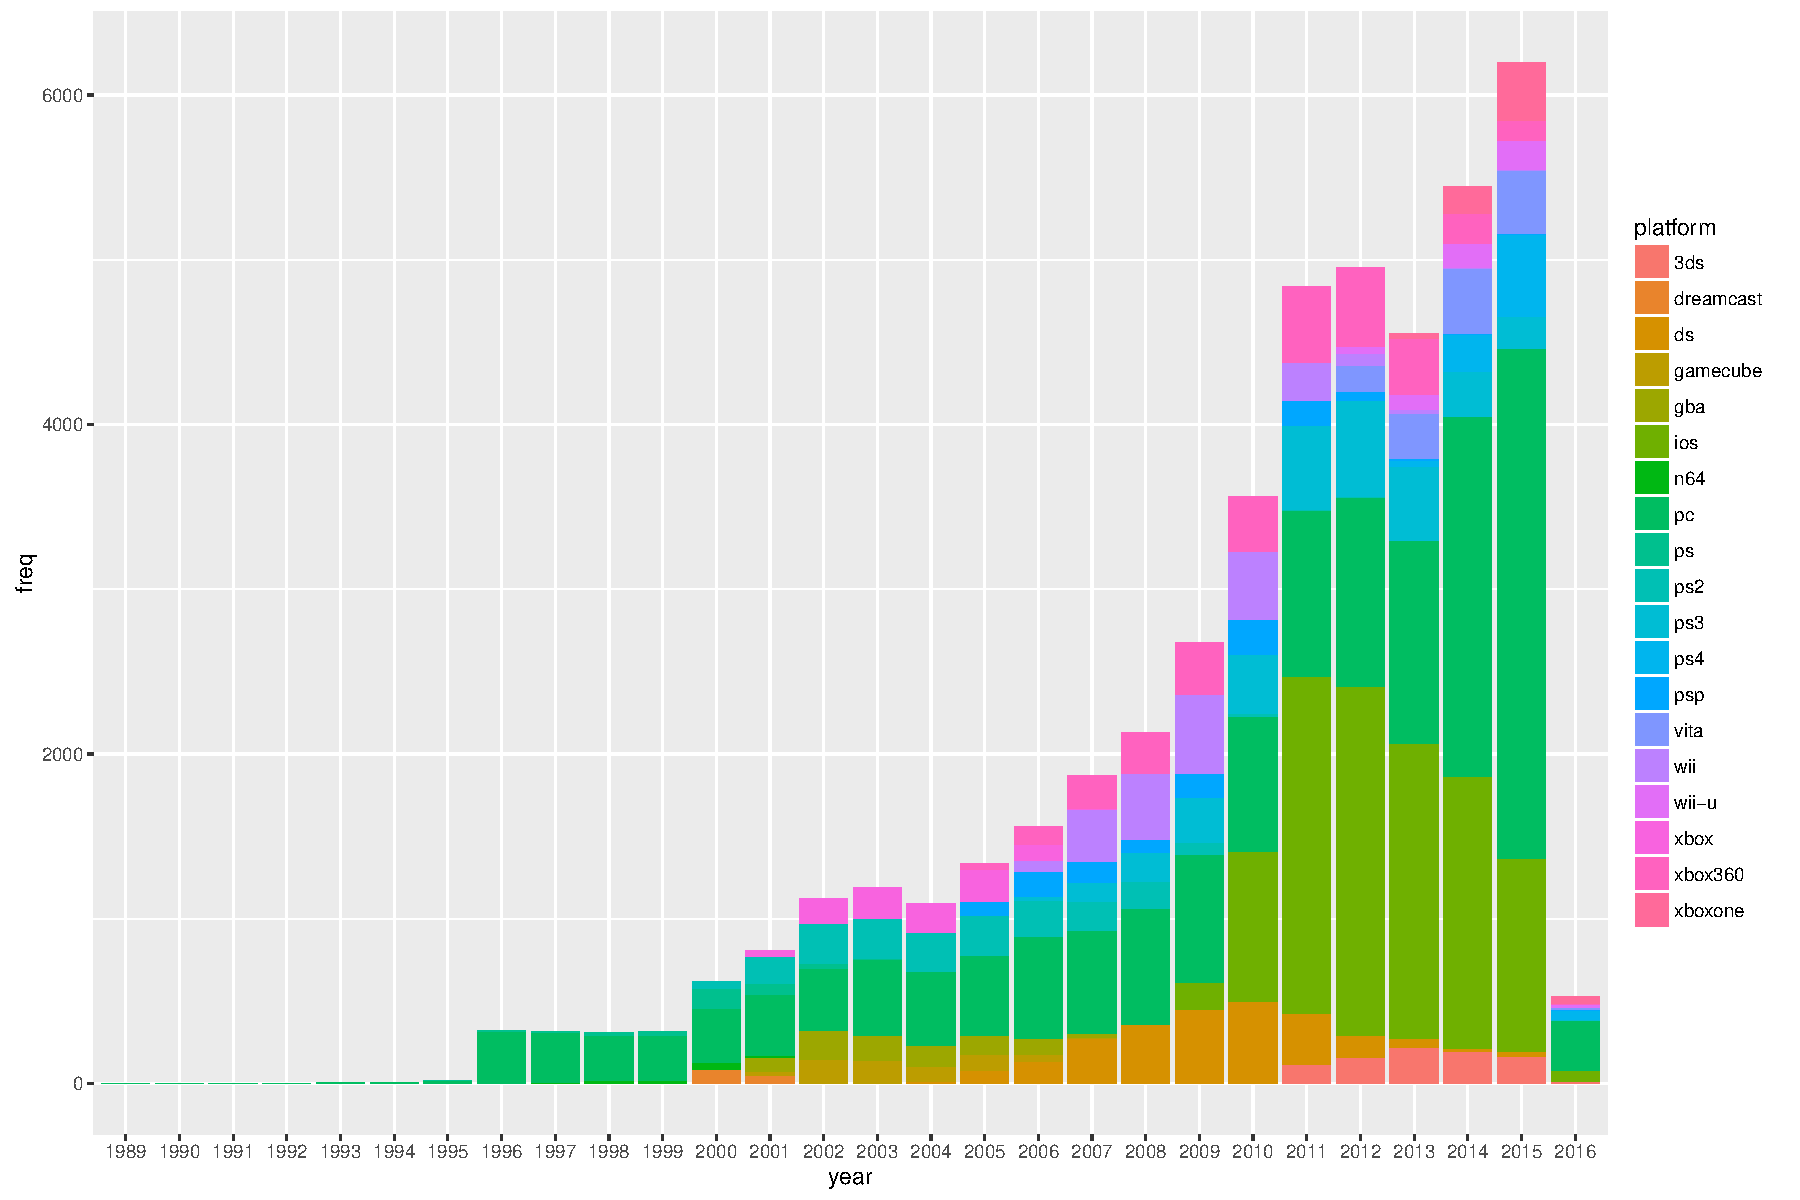
\includegraphics[width=1.0\columnwidth]{images/releases-per-year.pdf}
% 	\caption{Number of game releases per platform according to the Metacritic data.}
% \label{fig:releases-per-year}
% \end{figure}




